% --------------------------------------------------------------------------
% Report template for BIR projects
% Report template with support for Portuguese and English languages
% Change language {brazil or english} in \documentclass as per the examples
% This template has support for the ABNT citing format
%
% Original version: jan/2019
% https://github.com/
%
% Based on ABNTEX2 and the thesis template
% --------------------------------------------------------------------------
\documentclass[
%\DeclareUnicodeCharacter{200B}{}
% --------------------------------------------------------------------------
% classe memoir . options
12pt,					% tamanho da fonte
openright,				% cap. começam em pág ímpar (ins pág vazia caso preciso)
twoside,				% para impressão em verso e anverso. Oposto a oneside
a4paper,				% tamanho do papel
% --------------------------------------------------------------------------
% classe abntex2 . options
%chapter=TITLE,			% títulos de capítulos convertidos em letras maiúsc.
%section=TITLE,			% títulos de seções convertidos em letras maiúsc.
%subsection=TITLE,		% títulos de subseções convertidos em letras maiúsc.
%subsubsection=TITLE,	% títulos de subsubseções convertidos em letras maiúsc.
% --------------------------------------------------------------------------
% Opções de IDIOMA do pacote babel
english,
brazil
]{ABNT/abntex2_report}
% --------------------------------------------------------------------------
% Pacotes básicos
\usepackage{lmodern}			% Usa a fonte Latin Modern
\usepackage[T1]{fontenc}		% Seleção de códigos de fonte.
\usepackage[utf8]{inputenc}		% Codificação do documento (conversão automática dos acentos)
\usepackage{indentfirst}		% Indenta o primeiro parágrafo de cada seção.
\usepackage{color}				% Controle das cores
\usepackage{graphicx}			% Inclusão de gráficos
\usepackage{microtype} 			% para melhorias de justificação
\usepackage{lipsum}
\usepackage[brazilian,hyperpageref]{backref} % páginas com citações na bibliog.
%\usepackage[alf,abnt-etal-list=0,abnt-etal-cite=3,abnt-emphasize=bf]{abntex2cite}
\usepackage[alf]{abntex2cite}
%
\usepackage{lastpage}			% Usado pela Ficha catalográfica
%\usepackage{subfig}
\usepackage{supertabular}       % tabela na capa do documento
\usepackage{booktabs}
\usepackage[table,xcdraw]{xcolor}
\usepackage{adjustbox}
\usepackage{amssymb,amsmath,mathrsfs}
\usepackage{algorithm,algpseudocode}
\usepackage{pgfplots}
\usepackage{tikz}
\usepackage{titlesec}
\usepackage{ragged2e}
\usepackage{tocloft}
\usepackage{threeparttable}
\usepackage{etoolbox}
\usepackage[normalem]{ulem}
\usepackage{yaacro}
\usepackage[none]{verlab}
%\usepackage{fontspec}
%\setmainfont{Helvetica Light}
\usepackage{lscape}
%\usepackage[graphicx]{realboxes}
\usepackage{rotating}
\usepackage{wrapfig}
\usepackage{caption}
\usepackage{subcaption}
\usepackage{dirtytalk}
\usepackage{pdfpages}
\usepackage{threeparttable}
\usepackage{hyperref}
%\hypersetup{draft}
\usepackage{float}
\usepackage{listings}
\DeclareUnicodeCharacter{200B}{}
% --------------------------------------------------------------------------%
% Configurações do PDF final
\definecolor{blue}{RGB}{41,5,195}
\makeatletter
\hypersetup{
	%pagebackref=true,
	pdftitle={\@title},
	pdfauthor={\@author},
	pdfsubject={\@title},
	%pdfsubject={\imprimirpreambulo},
	pdfcreator={LaTeX with abnTeX2},
	pdfkeywords={abnt}{latex}{abntex}{abntex2}{\imprimirpalavraschave},
	colorlinks=true,       		% false: boxed links; true: colored links
	linkcolor=blue,          	% color of internal links
	citecolor=blue,        		% color of links to bibliography
	filecolor=magenta,      	% color of file links
	urlcolor=blue,
	bookmarksdepth=4
}
%\makeatother
% --------------------------------------------------------------------------
% Posiciona figuras e tabelas no topo da página quando adicionadas sozinhas
% em um página em branco. Ver https://github.com/abntex/abntex2/issues/170
%\makeatletter
\setlength{\@fptop}{5pt} % Set distance from top of page to first float
\makeatother
% --------------------------------------------------------------------------
% Formatação
\newcommand\tab[1][1cm]{\hspace*{#1}}
\apptocmd{\thebibliography}{\justifying}{}{}
\renewcommand{\ABNTEXsectionfont}{\bfseries}
\titlespacing*{\chapter}{0pt}{0pt}{12pt}
\titlespacing*{\section}{0pt}{6pt}{6pt}
\titlespacing*{\subsection}{0pt}{6pt}{6pt}
\titlespacing*{\subsubsection}{0pt}{6pt}{6pt}
% --------------------------------------------------------------------------
% Rearranja os finais de cada estrutura
\algrenewtext{EndWhile}{\algorithmicend\ \algorithmicwhile}
\algrenewtext{EndFor}{\algorithmicend\ \algorithmicfor}
\algrenewtext{EndIf}{\algorithmicend\ \algorithmicif}
\algrenewtext{EndFunction}{\algorithmicend\ \algorithmicfunction}
% --------------------------------------------------------------------------
% Espaçamentos entre linhas e parágrafos
\setlength{\parindent}{1.3cm} % linha
\setlength{\parskip}{0.2cm} % parágrafo, tente também \onelineskip
% --------------------------------------------------------------------------
% Informações de dados para CAPA e FOLHA DE ROSTO
\prodtecnica{001 / 2020}
\titulo{\textit{Design of Experiments}}
\tiporelatorio{Final}
\nomeprojeto{Modelagem do Helicóptero de Papel}
\outrossubtitulos{~} % opcional
\autores{
	Diogo Alexandre Martins\\
	Israel Cerqueira Motta Neto\\
	Mateus Santos de Cerqueira\\
	Pedro Paulo Ventura Tecchio
}
% \newcommand{\autoresexternos}{
% 	John Marston\\
% 	Frank West\
% }
\local{Salvador\\Bahia, Brasil}
\data{Setembro de 2020}
% \classificacao{( ) Confidencial  (X) Restrito  ( )  Uso Interno  ( ) Público}
% \revisao{01}
% \tabelacutter{000}
% \palavraschave{1. Manipulator. 2. Simulation. 3. Computer vision.}
% \classificacaoassunto{000} % sNúmero de Classificação do assunto
%\parceirologo{logos/x.png}
%------------------------------------------------------------------
% Finalização das configurações da capa
%
%
%------------------------------------------------------------------
% Acrônimos :: Chamar no texto como \ac{DoF}
\begin{acgroupdef}[list=acronyms]
	\acdef{DOE}{\textit{Design of Experiments}}
	%
	%
\end{acgroupdef}
% --------------------------------------------------------------------------
% Criação do sumário
\makeindex
%
\begin{document}
	% \frenchspacing
	\imprimircapa
	% \imprimircatalografica
% --------------------------------------------------------------------------
% Sumário executivo
	% \ABNTEXchapterfont\large\textbf{\execsummarytitlename}
	% \begin{flushleft}
	% 	\normalsize
	% 	\justify
	% 	\normalfont
	% 	O projeto de XXXX

	% 	O projeto iniciou no dia XX de XX de 20XX.

	% 	O prazo de execução planejado é de XX meses.
	% \end{flushleft}
	% \clearpage
%------------------------------------------------------------------
% Resumo e abstract
	\ABNTEXchapterfont\large\textbf{\resumoatitlename}
	\begin{flushleft}
		\normalsize
		\justify
		\normalfont
	Este relatório

	\end{flushleft}
\vspace*{1cm}
\newpage
	% %
	% \ABNTEXchapterfont\large\textbf{\resumobtitlename}
	% \begin{flushleft}
	% 	\normalsize
	% 	\justify
	% 	\normalfont
	% 	%abstract aqui
	% 	%
	% 	%
	% 	%
	% \end{flushleft}
	% \clearpage
% --------------------------------------------------------------------------
% Lista de figuras
	\begin{flushleft}
		\ABNTEXchapterfont\Large\textbf{\MakeUppercase\listadefigurasname}
	\end{flushleft}
	\vspace*{-36pt}
	\pdfbookmark[0]{\listfigurename}{lof}
	\normalsize
	\listoffigures*
	\cleardoublepage
% --------------------------------------------------------------------------
% Lista de tabelas
	\begin{flushleft}
		\ABNTEXchapterfont\Large\textbf{\MakeUppercase\listadetabelasname}
	\end{flushleft}
	\vspace*{-36pt}
	\pdfbookmark[0]{\listtablename}{lot}
	\normalsize
	\listoftables*
	\cleardoublepage
% --------------------------------------------------------------------------
% Lista de símbolos e abreviaturas
	% \begin{flushleft}
	% \ABNTEXchapterfont\Large\textbf{\MakeUppercase\listadesimbolsabrevtitlename}
	% 	\noindent
	% 	\vspace*{-06pt}
	% 	\pdfbookmark[0]{\listadesiglasname}{lot}
	% 	\normalsize
	% 	\normalfont
	% 	\aclist[list=acronyms]
	% \end{flushleft}
	% \newpage
% --------------------------------------------------------------------------
% Tabela de conteúdo
	\begin{flushleft}
		\ABNTEXchapterfont\Large\textbf{\MakeUppercase\glosariotitlename}
	\end{flushleft}
	%\pagebreak
	\vspace*{-36pt}
	\pdfbookmark[0]{\contentsname}{toc}
	\normalsize
	\normalfont
	\tableofcontents*
	\justify
--------------------------------------------------------------------------
% Formatação, remover espaço depois dos títulos
	\setlength\beforechapskip{-24pt}
	\setlength\afterchapskip{12pt}
	\textual
	\pagestyle{plain}
	\normalsize
	\justify
	\normalfont
% --------------------------------------------------------------------------
% Conteúdo do relatório
	\chapter{INTRODUÇÃO}
\label{chap:intro}
Para obter a construção do melhor modelo de helicóptero a base de papel, produzido seguindo o modelo da figura \ref{fig:modeloA4}, impresso no papel A4, a equipe borgs, desenvolveu um protótipo e realizou alguns lançamentos do modelo citado para analisar sua eficiência, avaliar qual a melhor configuração para que o modelo permaneça mais tempo no ar e analisar quais características podem interferir no desempenho de sua função. Após finalizado os lançamentos, foi gerada uma tabela com os tempos de lançamento de cada experimento.  A partir daí, foi realizada uma análise estatística utilizando o software R, no qual foi gerada as tabelas de comportamento gerado pela variação da altura e dos tipos de configuração física do protótipo.

\begin{figure}[H]
    \centering
    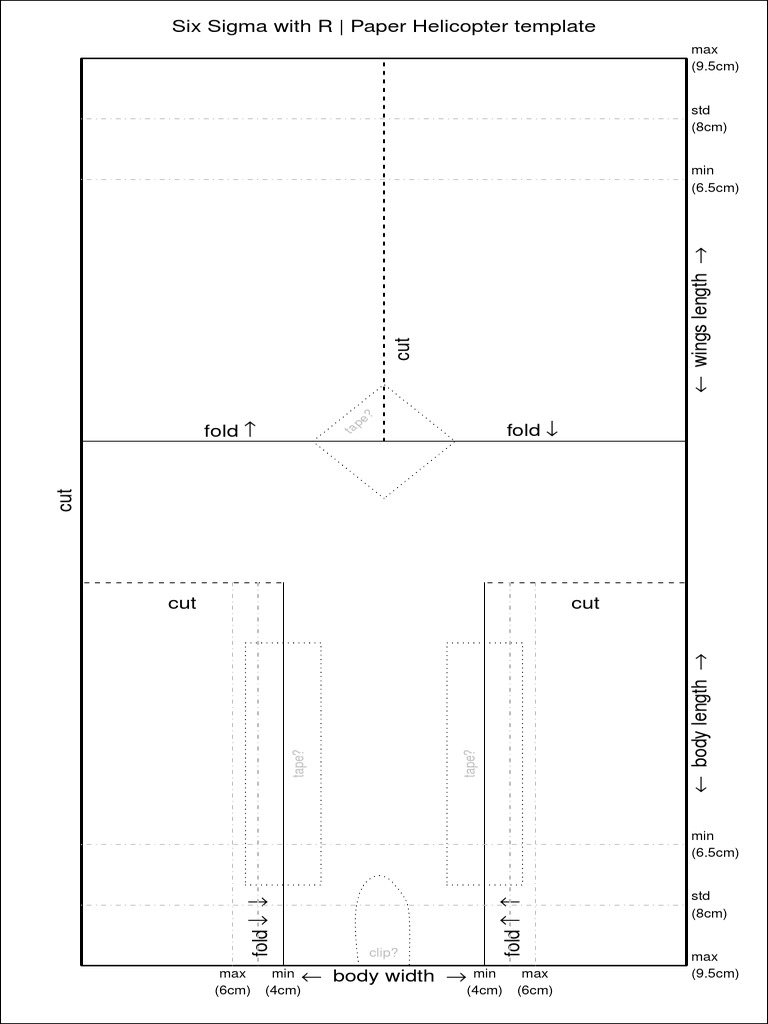
\includegraphics[scale=0.4]{images/helicoptero.jpeg}
    \caption{Cadeia de suprimentos.}
    \label{fig:modeloA4}
  \end{figure}

%------------------------------------------------------------------

\section{Objetivos}
\label{sec:obj}
Este trabalho tem como objetivo principal a criação, desenvolvimento e analise de um helicóptero impresso. O estudo do comportamento estatístico do modelo analisado, modelo matemático de tendência, repetitividade e reprodutividade foram feitos para aplicação e confirmação do experimento proposto.

%------------------------------------------------------------------
\section{Organização do relatório}
\label{sec:org}
Este documento está organizado da seguinte forma:
\begin{enumerate}
    \item Descrição do experimento, explicação da construção do modelo, análise e coleta de dados, padronização do teste e as variações que foram aplicadas; 
    \item Primeiro experimento, descrição das coleta de dados, tomada e aplicação em uma tabela;
    \item Modelagem matemática, aplicação dos dados coletados em um modelo matemático, explicação do que foi usado para análisar e o que foi gerado da analise feita;
    \item Segundo experimento, descrição das coleta de dados, tomada e aplicação em uma tabela;
    \item Verificação do experimento, confirmação dos dados;
    \item Conclusão, compreensão sobre o trabalho que foi apresentado.
    
\end{enumerate}
	\chapter{Descrição do Experimento}
\label{chap:descricao_do_experimento}

%! Escrever um pouco sobre o que é o experimento e qual o intuito

\section{O modelo utilizado}
\label{sec:o_modelo_utilizado}

%! Escrever sobre o helicoptero de papel e suas possíveis variáveis

\section{As variáveis escolhidas do modelo}
\label{sec:as_variavies_escolhidas_do_modelo}

%! Escrever sobre as variáveis que foram testadas e as expectativas das suas influências -> se colocar o clipe, o peso aumenta e possivelmente o tempo de voo diminui etc...
	\chapter{Primeiro Experimento}
\label{chap:primeiro_experimento}

%! Escrever um pouco sobre o que foi feito

\section{Criando o experimento no R}
\label{sec:primeiro_experimento_criando o experimento_no_R}

%! Escrever sobre código usado para criar o experimento, a sequencia de testes, no R. Qual o motivo de usar isso?


\begin{table}[H]
  \centering
  \caption{Experimento de modelagem do helicóptero de papel.}
  \resizebox{0.7\textwidth}{!}{%
  \begin{tabular}{c|c|c|c}
  \textbf{Altura} & \textbf{Clipe} & \textbf{AdesivoTopo} & \textbf{AdesivoLateral} \\ \hline
  1.3             & -              & +                    & +                       \\ \hline
  2.1             & +              & +                    & -                       \\ \hline
  1.3             & -              & -                    & +                       \\ \hline
  2.1             & +              & -                    & -                       \\ \hline
  1.3             & +              & -                    & -                       \\ \hline
  2.1             & -              & +                    & -                       \\ \hline
  2.1             & -              & -                    & -                       \\ \hline
  1.3             & +              & +                    & +                       \\ \hline
  2.1             & -              & -                    & +                       \\ \hline
  1.3             & -              & -                    & -                       \\ \hline
  2.1             & +              & +                    & +                       \\ \hline
  2.1             & +              & -                    & +                       \\ \hline
  2.1             & -              & +                    & +                       \\ \hline
  1.3             & -              & +                    & -                       \\ \hline
  1.3             & +              & -                    & +                       \\ \hline
  1.3             & +              & +                    & -
  \end{tabular}%
  }
  \legend{Fonte: Autores.}
  \label{tab:experimento_modelagem_helicoptero_papel}
\end{table}

\section{A coleta de dados}
\label{sec:primeiro_experimento_a_coleta_de_dados}

%! Escrever sobre como foi feita a coleta de dados e indicar a tabela resultante
	\chapter{A Modelagem Matemática}
\label{chap:a_modelagem_matematica}

%! Escrever um pouco sobre o que foi feito

\section{Utilizando o modelo linear}
\label{sec:a_modelagem_matematica_utilizando_o_modelo_linear}

%! Escrever sobre código usado para criar o modelo linear, como este é capaz de utilizar não linearidades

\section{O modelo resultante}
\label{sec:a_modelagem_matematica_o_modelo_resultante}

%! Escrever sobre o resultado encontrado e o que ele nos informa
	\chapter{Segundo Experimento}
\label{chap:segundo_experimento}

%! Escrever um pouco sobre o que foi feito

\section{Criando o experimento no R}
\label{sec:segundo_experimento_criando o experimento_no_R}

%! Escrever sobre código usado para criar o experimento, a sequencia de testes, no R. Qual o motivo de usar isso?

\section{A coleta de dados}
\label{sec:segundo_experimento_a_coleta_de_dados}

%! Escrever sobre como foi feita a coleta de dados e indicar a tabela resultante
	\chapter{Verificação do Modelo}
\label{chap:verificacao_do_modelo}

%! Escrever um pouco sobre o que foi feito
Após a comprovação de que as variáveis $Clipe$ e $Altura$ são as mais significativas na criação do primeiro modelo, foi criado um modelo linear de primeira ordem contemplando somente estas duas variávei, utilizando os dados medidos para teste. Os coeficientes obtidos utilizando o modelo linear são mostrados na Tabela~\ref{tab:terc-mod}.

% latex table generated in R 4.0.2 by xtable 1.8-4 package
% Mon Sep 21 23:47:47 2020
\begin{table}[ht]
    \centering
    \caption{Modelo linear de primeira ordem.}
    \begin{tabular}{rrrrr}
      \hline
     & Estimate & Std. Error & t value & Pr($>$$|$t$|$) \\ 
      \hline
    (Intercept) & -0.0967 & 0.0745 & -1.30 & 0.2012 \\ 
      Altura & 0.8563 & 0.0416 & 20.59 & 0.0000 \\ 
      Clipe+ & -0.1100 & 0.0333 & -3.31 & 0.0019 \\ 
       \hline
    \end{tabular}
    \label{tab:terc-mod}
    \end{table}

No modelo testado, os valores obtidos estão situados em uma faixa entre -0.40146 e 0.28854, e a mádia de todos os valores atinge um valor de 0.00354. Os gráficos gerados utilizando este modelo mostrando os residuais estão representados na Figura~\ref{fig:residuos-plot3}.

\begin{figure}[H]
    \centering
    \caption{Gráficos dos resíduos do modelo linear.}
    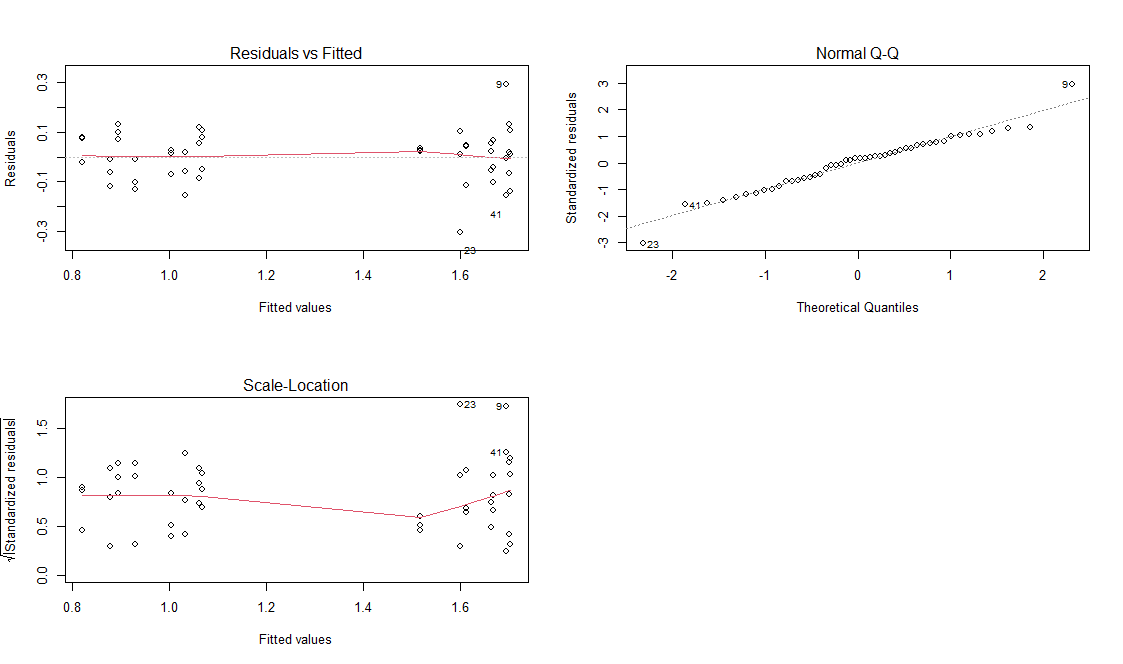
\includegraphics[width=0.8\textwidth]{images/model.png}
    \legend{Fonte: Autores.}
    \label{fig:residuos-plot3}
  \end{figure}

  No modelo gerado, foi obtido um valor de $R^2$ múltiplo de 0.9062, ou seja, o modelo pode explicar 90.62\% da variabilidade total, e o valor obtido do $R^2$ ajustado é 0.902. 

\section{Utilizando a correlação de dados}
\label{sec:verificacao_do_modelo_utilizando_a_correlacao_de_dados}

%! Escrever sobre código usado para correlacionar os dados preditos com os encontrados no segundo experimento

Em seguida, foram utilizados como dados de entrada as alturas utilizadas no segundo experimento, e em seguida submetidas ao modelo gerado no primeiro experimento. Em seguida, os resultados obtidos com esta predição foram comparadas aos dados empíricos obtidos no segundo experimento, utilizando a correlação de Pearson. 

\section{O resultado}
\label{sec:verificacao_do_modelo_o_resultado}

%! Escrever sobre o resultado encontrado e o que ele nos informa

O resultado encontrado indica que o modelo gerado no experimento foi capaz de obter uma correlação de 0.9880744 com os testes empíricos. Estes experimentos significam que o modelo gerado foi capaz de descrever o helicóptero com um modelo matemático que se assemelha bastante aos resultados reais, obtidos em teste. Os gráficos gerados da correlação, comparando as predições feitas no primeiro modelo com os resultados dos testes estão representados na Figura~\ref{fig:corr}.

\begin{figure}[H]
    \centering
    \caption{Gráficos da correlação entre o modelo gerado e testes empíricos.}
    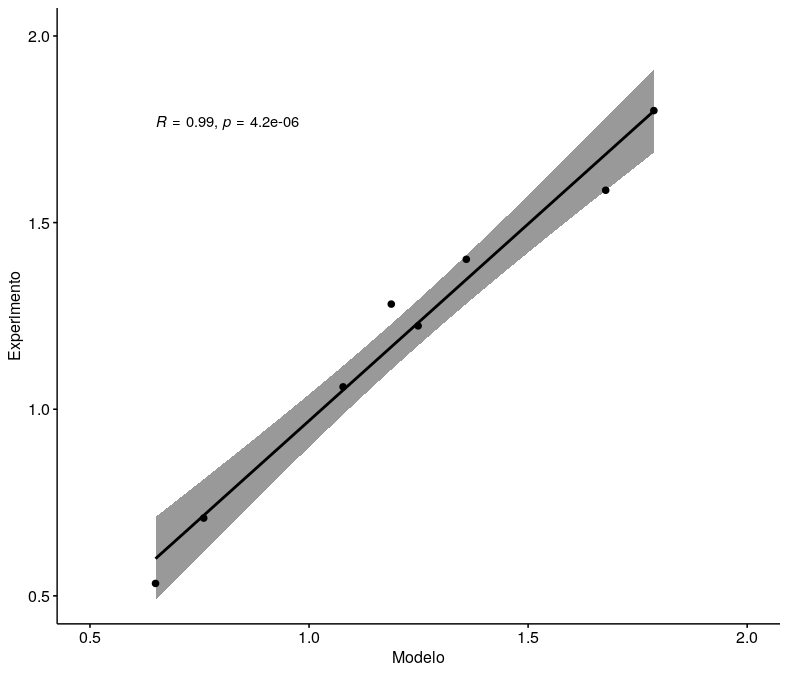
\includegraphics[width=0.8\textwidth]{images/corr.png}
    \legend{Fonte: Autores.}
    \label{fig:corr}
  \end{figure}
	\chapter{CONCLUSÃO}
\label{chap:conclusao}

Este trabalho apresentou ...

% --------------------------------------------------------------------------
% Referências
	% \cleardoublepage
	\titleformat{\chapter}[display]{\vspace*{-24pt}\ABNTEXchapterfont\large\bfseries}{\chaptertitlename\ \thechapter}{12pt}{\Large}
	\bibliography{bibliography}
% --------------------------------------------------------------------------
% Apêndices
\apendices
\justify
\chapter{Tabelas de dados dos experimentos}
\label{chap:app_tabelas_de_dados_dos_experimentos}

Os dados experimentais encontrados para o tempo de vôo do modelo de helicóptero de papel estão apresentados a seguir. A Seção \ref{sec:app_experimento_1} - Experimento 1 apresenta os resultados obtidos a partir dos experimentos gerados na Seção \ref{sec:primeiro_experimento_criando o experimento_no_R} e apresentados na Tabela \ref{tab:experimento_modelagem_helicoptero_papel}. Analogamente, a Seção \ref{sec:app_experimento_2} - Experimento 2 apresenta os dados encontrados para o experimento da Seção \ref{sec:segundo_experimento_criando o experimento_no_R} e apresentados na Tabela \ref{tab:experimentos_para_teste_do_modelo}.

\section{Experimento 1}
\label{sec:app_experimento_1}

\begin{table}[H]
  \caption{Dados experimentais para modelagem.}
  \resizebox{\textwidth}{!}{%
  \begin{tabular}{c|c|c|c|c|c}
  \textbf{Teste1\_Mateus} & \textbf{Teste1\_Pedro} & \textbf{Teste2\_Mateus} & \textbf{Teste2\_Pedro} & \textbf{Teste3\_Mateus} & \textbf{Teste3\_Pedro} \\ \hline
  0.90 & 1.05 & 0.73 & 1.03 & 1.12 & 0.98 \\ \hline
  1.61 & 1.61 & 1.71 & 1.73 & 1.59 & 1.79 \\ \hline
  1.22 & 1.14 & 1.18 & 1.05 & 1.02 & 0.93 \\ \hline
  1.61 & 1.47 & 1.52 & 1.59 & 1.54 & 1.55 \\ \hline
  0.86 & 0.93 & 0.84 & 0.76 & 0.88 & 0.92 \\ \hline
  1.60 & 1.67 & 1.78 & 1.66 & 1.82 & 1.85 \\ \hline
  1.70 & 1.71 & 1.35 & 1.25 & 1.56 & 1.66 \\ \hline
  0.95 & 0.98 & 1.13 & 0.92 & 0.94 & 1.05 \\ \hline
  1.98 & 2.00 & 1.75 & 1.63 & 1.52 & 1.56 \\ \hline
  1.02 & 1.02 & 1.04 & 1.02 & 0.96 & 0.91 \\ \hline
  1.47 & 1.66 & 1.63 & 1.62 & 1.82 & 1.65 \\ \hline
  1.55 & 1.45 & 1.60 & 1.72 & 1.71 & 1.60 \\ \hline
  1.69 & 1.74 & 1.79 & 1.83 & 1.53 & 1.60 \\ \hline
  1.15 & 1.14 & 0.94 & 1.10 & 1.20 & 1.15 \\ \hline
  0.82 & 0.92 & 0.83 & 0.80 & 0.76 & 0.76 \\ \hline
  0.93 & 0.73 & 0.79 & 0.81 & 0.92 & 0.92
  \end{tabular}%
  }
  \legend{Fonte: Autores.}
  \label{tab:dados_experimentais_para_modelagem}
\end{table}

\section{Experimento 2}
\label{sec:app_experimento_2}

\begin{table}[H]
  \caption{Dados experimentais para teste do modelo.}
  \resizebox{\textwidth}{!}{%
  \begin{tabular}{c|c|c|c|c|c}
  \textbf{Teste1\_Mateus} & \textbf{Teste1\_Pedro} & \textbf{Teste2\_Mateus} & \textbf{Teste2\_Pedro} & \textbf{Teste3\_Mateus} & \textbf{Teste3\_Pedro} \\ \hline
  1.40 & 1.40 & 1.52 & 1.43 & 1.27 & 1.39 \\ \hline
  1.28 & 1.22 & 1.12 & 1.12 & 1.30 & 1.30 \\ \hline
  0.69 & 0.60 & 0.74 & 0.82 & 0.72 & 0.68 \\ \hline
  0.55 & 0.63 & 0.43 & 0.48 & 0.51 & 0.60 \\ \hline
  1.57 & 1.50 & 1.58 & 1.65 & 1.53 & 1.69 \\ \hline
  1.25 & 1.10 & 0.95 & 0.90 & 1.13 & 1.03 \\ \hline
  1.18 & 1.25 & 1.36 & 1.36 & 1.22 & 1.32 \\ \hline
  1.67 & 1.65 & 1.95 & 1.85 & 1.83 & 1.85
  \end{tabular}%
  }
  \legend{Fonte: Autores.}
  \label{tab:dados_experimentais_teste_modelo}
\end{table}
\chapter{Código completo utilizado}
\label{chap:app_codigo_completo_utilizado}

\section{Geração do experimento de modelagem}
\label{sec:app_codigo_geracao_do_experimento_de_modelagem}

\lstinputlisting[language=R,inputencoding=latin1]{code/helicoptero_cria_experimento_modelagem.R}


\section{Geração do experimento de teste do modelo}
\label{sec:app_codigo_geracao_do_experimento_de_teste_do_modelo}

\lstinputlisting[language=R,inputencoding=latin1]{code/helicoptero_cria_experimento_teste_modelo.R}


\section{Análise dos dados}
\label{sec:app_codigo_analise_dos_dados}

\lstinputlisting[language=R,inputencoding=latin1]{code/helicoptero_teste_media.R}
% %

% --------------------------------------------------------------------------
% % Anexos
% \anexos
% \justify
% \include{annex/XXyyyy}
% %
\end{document}